\newpage{}
\section{Deep Reinforcement Learning}


%============================================
\subsection{Motivation}
\subsubsection{Why RL}
Making sequences of decisions.

Delayed labels. After you take the action, you will know the result.


\subsubsection{What is RL}
Automatically learn to make good sequences of decision.


\subsubsection{Examples}
Robotics

Games

Advertisement


%============================================
\subsection{Recycling Game}
\subsubsection{Q learning}
\begin{figure}[h!] % Here
	\centering
	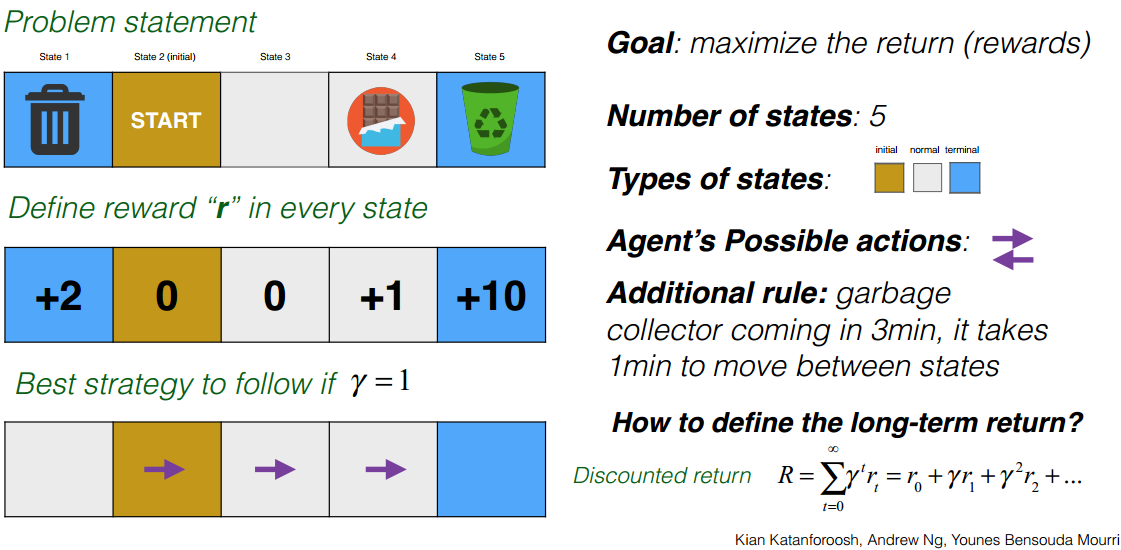
\includegraphics[width=1.0\linewidth]{img/recycling_game_0.png}
	\caption{Game}\label{img:recycling_game_0}
\end{figure}

\begin{figure}[h!] % Here
	\centering
	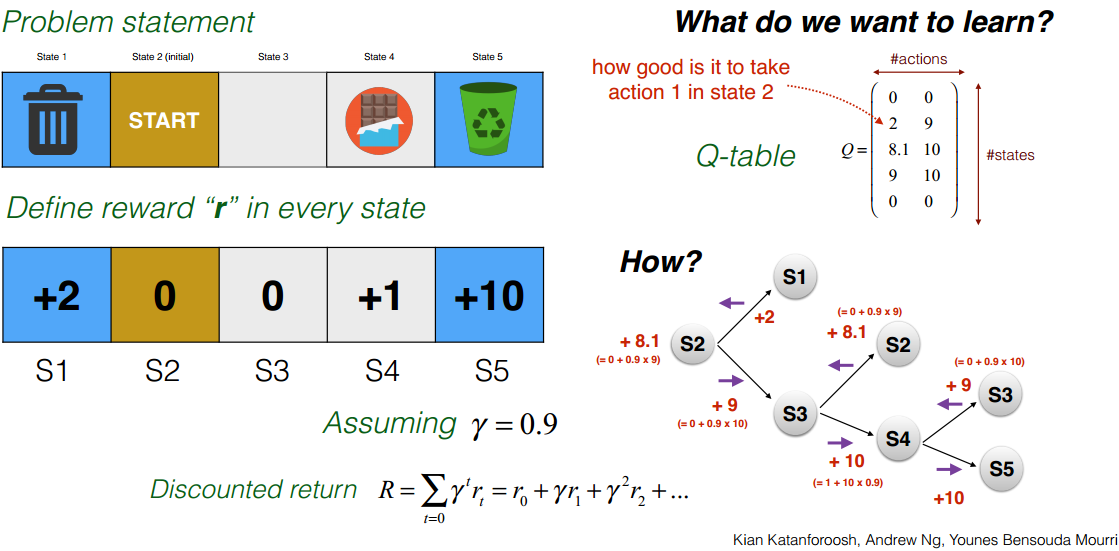
\includegraphics[width=1.0\linewidth]{img/recycling_game_1.png}
	\caption{Q-table}\label{img:recycling_game_1}
\end{figure}

\begin{figure}[h!] % Here
	\centering
	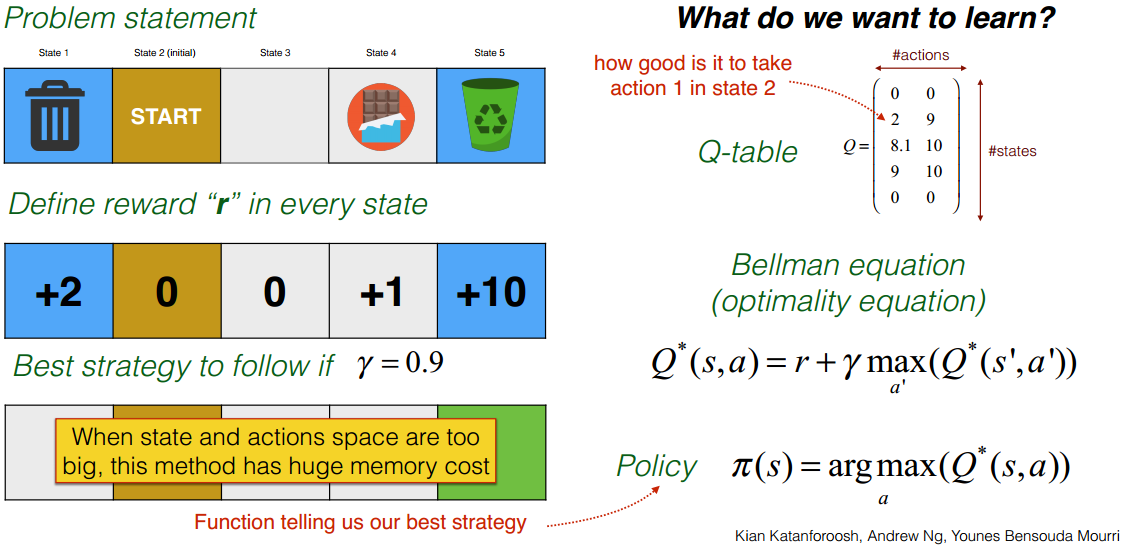
\includegraphics[width=1.0\linewidth]{img/recycling_game_2.png}
	\caption{Bellman equation and Policy}\label{img:recycling_game_1}
\end{figure}

\subsubsection{Summary}
Vocabulary: environment, agent, state, action, reward, total return, 
discount factor/discount rate.

Q-table: matrix of entries representing ``how good is it to take action a
in state s''

Policy: function telling us what's the best strategy to adopt

Bellman equation satisfied by the optimal Q-table


%============================================
\subsection{Deep Q-Networks}

\subsubsection{Main idea}
Main idea: find a Q-function to replace the Q-table

Q-function: Neural Network.

\subsubsection{Deep Q Learning}
\begin{align}
	\hat{y} &= Q(s, a) \\
	L &= (y - \hat{y})^2 \\
	y &= r + \gamma \displaystyle\max_{a'}(Q(s^{next}_a, a')) % // after taking a
\end{align}

Backpropagation:
Compute $\frac{\partial L}{\partial W}$ and update W using stochastic gradient descent.


%============================================
\subsection{Application of Deep Q-Network: Breakout (Ataria)}
\begin{itemize}
	\item Deep Q-network architecture: CNN for image input.
	\item Exploration vs. Exploitation
	\item Implementation:
	\begin{itemize}
		\item Preprocessing
		\item Detect terminal State
		\item Experience replay
		\item Epsilon greedy action
	\end{itemize}
\end{itemize}


%============================================
\subsection{Advanced topics}
Policy Gradient Methods: 
PPO(Proximal Policy Optimization), 
TRPO(Trust Region Policy Optimization).
